\documentclass[11pt]{article}

\usepackage[margin=1in, headheight=14.5pt]{geometry}
\usepackage{amsfonts, amsmath, amssymb}
\usepackage{enumitem}
\usepackage[none]{hyphenat}
\usepackage{fancyhdr}
\usepackage[spanish, es-noshorthands]{babel}
\usepackage[spanish, calc]{datetime2}
\usepackage{fmtcount}
\usepackage{graphicx}
\usepackage{float}
\usepackage[nottoc, notlot, notlof]{tocbibind}
\usepackage{tocloft}
\usepackage[utf8]{inputenc}
\usepackage{parskip}
\usepackage{xcolor}
\usepackage{cancel}
\usepackage{textcomp}
\usepackage{pgfplots}
\usepackage{tikz}
\usetikzlibrary{shapes.misc}
\usepackage{polynom}
\usetikzlibrary{datavisualization}
\usetikzlibrary{datavisualization.formats.functions}
\pgfplotsset{compat=1.15}
\usepackage{mathrsfs}
\usetikzlibrary{arrows}
\usepackage{adjustbox}

\newcommand{\dropsign}[1]{\smash{\llap{\raisebox{-.5\normalbaselineskip}{$#1$\hspace{2\arraycolsep}}}}}%


\parindent 0ex

\pgfplotsset{width=10cm,compat=1.9}

\def\imj{\mathrm{j}}
\def\sen{\mathrm{sen}}

\newcommand{\lapl}[1]{\mathscr{L} \left\lbrace {#1} \right\rbrace}
\newcommand{\ilapl}[1]{\mathscr{L}^{-1} \left\lbrace {#1} \right\rbrace}

\renewcommand\cftsecleader{\cftdotfill{\cftdotsep}}
\renewcommand{\baselinestretch}{1.1}
\newcommand*\circled[1]{\tikz[baseline=(char.base)]{
		\node[shape=circle,draw,inner sep=2pt] (char) {#1};}}
	
\newcommand{\highlight}[2]{\colorbox{#1}{$\displaystyle #2$}}

\graphicspath{{\ProjectRoot/commons/img/}}

\newcommand*{\ProjectRoot}{../../matematica-superior}


\begin{document}
		
	\begin{titlepage}
		\begin{center}
			\vspace*{0.5cm}
			\Large{\textbf{Universidad Tecnológica Nacional}}\\
			\Large{\textbf{Facultad Regional Buenos Aires}}\\
			\begin{center}
				
\includegraphics[scale=0.4]{logoutn.png}
			\end{center}
			\vfill
			\line(1,0){400}\\
			\vspace*{0.3cm}
			\huge{\textbf{Matemática Superior}}\\
			\Large{\textbf{Repaso segundo parcial}}\\
			\line(1,0){400}\\
			\vfill
			Tomás Moreira \\
			
			\DTMnewdatestyle{mydate}{%
				\renewcommand{\DTMdisplaydate}[4]{%
					\DTMMonthname{##2} \number##1
				}
				\renewcommand{\DTMDisplaydate}{\DTMdisplaydate}
			}
			
			\DTMsetdatestyle{mydate}
			\today
				
				
		\end{center}
	\end{titlepage}

	\tableofcontents
	\thispagestyle{empty}
	\clearpage

	\setcounter{page}{1}
	
	\textbf{\Large{Parcial tomado en junio de 2017}}
	\section{Ejercicio Raíces de ecuaciones no lineales}
	Dada la ecuación $\sen(3x)-x^2+3=0$
	
	\begin{enumerate}[label=\alph*)]
		\item Indique un intervalo de longitud menor o igual a 1 para cada una de las raíces de la ecuación.
		\item Sabiendo que una de las raíces es negativa, se proponen 2 valores iniciales: $x_0=-1.3$ y $x_0=-1,9$. Calcule dicha raíz con $\varepsilon<10^{-5}$ utilizando el método de Newton-Raphson, utilizando uno de los valores iniciales propuestos. Justifique su elección del valor inicial de modo que se minimicen la cantidad de iteraciones.
	\end{enumerate}

	\textbf{Inciso a}
	
	Recordemos, para resolver esta parte del ejercicio habría que hacer un gráfico de las funciones:
	
	$\sen(3x)=x^2-3$
	
	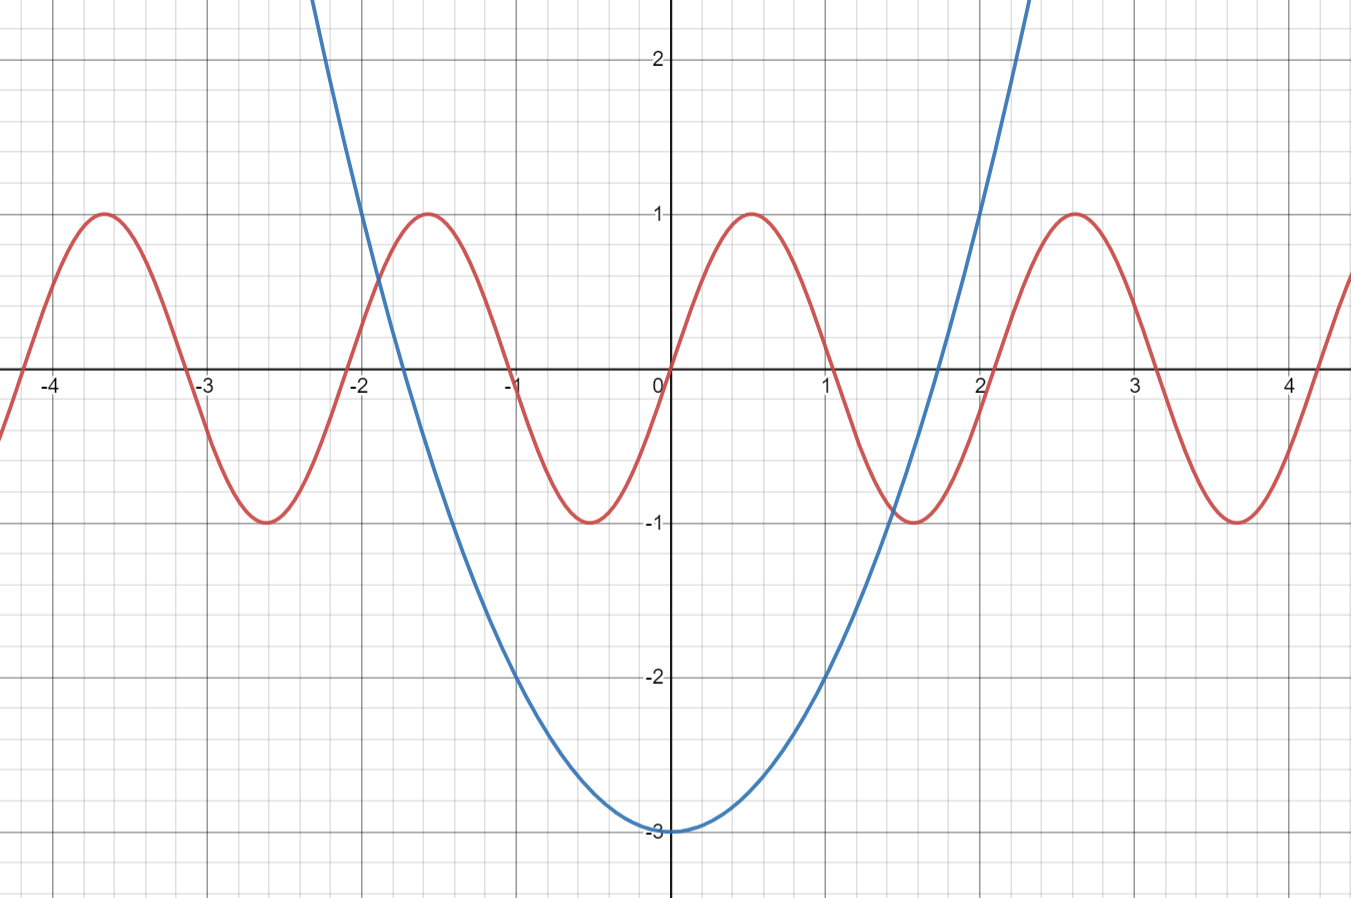
\includegraphics[scale=0.6]{2p/raices.png}
	
	Vemos que hay dos raíces, ubicadas en el $[-2;-1]$ y el $[1;2]$\\
	
	\textbf{Inciso b}
	
	Vamos a derivar nuestra función asociada a la ecuación: $f(x)=\sen(3x)-x^2+3$
	
	$f'(x)=3\cos(3x)-2x$
	
	Si evaluamos los dos puntos en esta derivada, obtenemos:
	
	$f'(-1.9)=6.304138355$
	
	$f'(-1.3)=0.4222030874$
	
	Vemos que para $x=-1.3$ la derivada está peligrosamente cercana a 0, por lo que es muy probable que cerca se encuentre un extremo local. En cambio, para $x=-1.9$ tenemos un número grande (que nos viene excelente). Así que vamos a usar $x_0=-1.9$
	
	Aplicando la fórmula de Newton:
	
	$\displaystyle x_{i+1}=x_i-\frac{f(x_i)}{f'(x_i)}$
	
	$\displaystyle x_{i+1}=x_i-\frac{\sen(3x_i)-x_i^2+3}{3\cos(3x_i)-2x_i}$
	
	$\displaystyle x_1=-1.9-\frac{\sen(3\cdot(-1.9))-(-1.9)^2+3}{3\cos(3\cdot(-1.9))-2\cdot(-1.9)}=-1.890591187$
	
	$\displaystyle x_2=-1.890591187-\frac{\sen(3\cdot(-1.890591187))-(-1.890591187)^2+3}{3\cos(3\cdot(-1.890591187))-2\cdot(-1.890591187)}=-1.890541327$
	
	$\displaystyle x_3=-1.890541327-\frac{\sen(3\cdot(-1.890541327))-(-1.890541327)^2+3}{3\cos(3\cdot(-1.890541327))-2\cdot(-1.890541327)}=-1.890541325 \rightarrow $ PARO.
	
	Cabe destacar que no es necesario aclarar uno por uno los valores y las iteraciones en cada paso. Lo hago nomás a modo de repaso, en el parcial alcanza con poner la fórmula que se va a usar y luego hacer una tabla con los $x_i$ sucesivos que se van obteniendo. A lo sumo especificar el primer paso.

	\section{Ejercicio Interpolación + Diferenciación numérica}
	Dada la siguiente tabla de valores:
	
	\begin{tabular}{|c|c|}
		\hline
		$x$ & $y$\\
		\hline
		1 & 1\\
		\hline
		2 & $k$\\
		\hline
		3 & 23\\
		\hline
		5 & 61\\
		\hline
		6 & 86\\
		\hline
	\end{tabular}

	\begin{enumerate}[label=\alph*)]
		\item Determine, si es posible, el valor de $k \in \mathbb{R}$ tal que el polinomio interpolante que pasa por todos los puntos sea de grado 2.
		\item En el caso de que $k=30$, determine de que grado es el polinomio sin realizar las tablas de diferencia.
		\item Hallar la primera diferencia en $x=4$
	\end{enumerate}

	\textbf{Inciso a}
	
	Nos piden un polinomio de grado 2, por ende vamos a usar 3 puntos para calcularlo.
	
	\begin{tabular}{|c c c c|}
		\hline
		$x_i$ & $y_i$ & O1 & O2\\
		\hline
		1 & 1 & & \\
		& & 11 & \\
		3 & 23  & &2 \\
		& & 19 & \\
		5  & 61 & & \\
		\hline
	\end{tabular}

	El polinomio interpolante, usando el progresivo es:
	
	$p(x)=1+11(x-1)+2(x-1)(x-3)$
	
	Si usaramos el regresivo sería:
	
	$p(x)=61+19(x-5)+2(x-5)(x-3)$
	
	Usamos el progresivo porque tiene números ``más lindos''. 
	
	Primero hay que verificar que el polinomio pase por los puntos que no consideramos al hacer la tabla reducida: ¿$p(6)=86$?
	
	$p(6)=1+11(6-1)+2(6-1)(6-3)=86 \rightarrow$ VERIFICA.
	
	Entonces, para hallar $k$ basta con hacer $p(2)$
	
	$p(2)=k \rightarrow k=1+11(2-1)+2(2-1)(2-3)=10$
	
	Por ende si $k=10$, por los puntos pasa un polnimoio de grado 2.\\
	
	\textbf{Inciso b}
	
	Si fuera $k=30$, el polinomio se sale del patrón de los puntos, que forman parte de un polinomio de grado 2. Cuando pasa esto, el polinomio se va al máximo grado posible. \textbf{Como tenemos 5 puntos, entonces el polinomio será de grado 4}.\\
	
	\textbf{Inciso c}
	
	Para hallar la primera diferencia en $x=4$ solo lo podemos hacer con la fórmula central, con $h=1$.
	
	$\displaystyle f'(4)=\frac{61-23}{2\cdot1}=\frac{38}{2}=19$
	
	\section{Ejercicio Integración numérica}
	Dada la integral $\displaystyle \int_{1}^{3}x^3\ln(x)dx$ indique la mínima cantidad de subintervalos en el $[1;3]$ de modo que al resolver la integral por Método de Simpson se asegure un $\varepsilon<10^{-2}$. Usando el resultado anterior calcula la integral por Simpson.
	
	Para resolver el ejercicio, debemos acotar el error. En este caso tenemos el método de Simpson, entonces primero vamos a derivar la función:
	
	$f(x)=x^3\ln(x)$
	
	$\displaystyle f'(x)=3x^2 \ln(x) + x^3\cdot \frac{1}{x}=3x^2\ln(x)+x^2$
	
	$\displaystyle f''(x)=6x\ln(x)+3x^2 \cdot \frac{1}{x}+2x=6x\ln(x)+5x$
	
	$\displaystyle f'''(x)=6\ln(x)+6x\cdot \frac{1}{x}+5=6\ln(x)+11$
	
	$\displaystyle f^{(IV)}=\frac{6}{x}$
	
	El máximo de esta función está en $x=1$, considerando nuestro intervalo de trabajo.
	
	$f^{(IV)}(1)=6$
	
	Con este valor, usamos la fórmula de error:
	
	$\displaystyle |e_S|=\left| \frac{b-a}{180} \right|h^4 \max_{a\le \xi \le b}  \left|f^{(IV)}(\xi) \right|<\varepsilon$
	
	$\displaystyle \left|\frac{3-1}{180}\right|h^4 \max_{1\le \xi \le 3}  \left|f^{(IV)}(\xi) \right|<10^{-2}$
	
	$\displaystyle \frac{2}{180} \cdot h^4 \cdot 6 < 10^{-2}$
	
	$\displaystyle h < \sqrt[4]{\frac{10^{-2}\cdot 180}{6\cdot2}}$
	
	$h < 0.6223329773$
	
	$\displaystyle N=\frac{b-a}{h}=\frac{3-1}{0.6223329773}=3.2137...$
	
	Como es Simpson, debemos tener en cuenta que necesitamos una cantidad PAR de subintervalos. Si probamos con $N=4$, obtenemos un $h$ muy cómodo:
	
	$\displaystyle h=\frac{b-a}{N}=\frac{2}{4}=\boxed{0.5}$
	
	Con ese $h$, hacemos la tabla para usar el método de Simpson.
	
	\begin{tabular}{|c|c|c|}
		\hline
		$i$ & $x_i$ & $f(x_i)$\\
		\hline
		0 & 1 & 0\\
		\hline
		1 & 1.5 & 1.36844\\
		\hline
		2 & 2 & 5.54518\\
		\hline
		3 & 2.5 & 14.31704\\
		\hline
		4 & 3 & 29.66253\\
		\hline
	\end{tabular}

	$\displaystyle I_S=\frac{h}{3}(E+4I+2P)$
	
	$\displaystyle I_S=\frac{0.5}{3}((0+29.66253)+4(1.36844+14.31704)+2(5.54518))=\boxed{17.249135}$
	
	\section{Ejercicio Sistemas de ecuaciones lineales}
	Dado el siguiente sistema de ecuaciones lineales:
	$\begin{cases}
		2x+5y+z=15\\
		2x-2y+6z=3\\
		7x+2y-3z=8
	\end{cases}$

	Ordenar el anterior sistema de modo que se pueda resolver por método iterativo. Realice dos iteraciones por el Método de Gauss-Seidel usando $x_0=(0,2,1)$\\
	
	Reordenamos de manera que la matriz de coeficientes asociada al sistema sea diagonal dominante:
	
	$\begin{cases}
		7x+2y-3z=8\\
		2x+5y+z=15\\
		2x-2y+6z=3
	\end{cases}$

	Realizamos el despeje de las ecuaciones y dejamos expresadas las fórmulas iterativas:

	$\displaystyle x_{i+1}=-\frac{2}{7}y_i+\frac{3}{7}z_i+\frac{8}{7}$
	
	$\displaystyle y_{i+1}=-\frac{2}{5}x_{i+1}-\frac{1}{5}z_i+\frac{15}{5}$
	
	$\displaystyle z_{i+1}=-\frac{2}{6}x_{i+1}+\frac{2}{6}y_{i+1}+\frac{3}{6}$
	
	Usando el valor inicial que nos dan como dato $x_0=(0,2,1)$ iteramos:
	
	$\displaystyle x_1=-\frac{2}{7}\cdot2+\frac{3}{7}\cdot 1+\frac{8}{7}=1$
	
	$\displaystyle y_1=-\frac{2}{5}\cdot1-\frac{1}{5}\cdot 1+\frac{15}{5}=2.4$
	
	$\displaystyle z_1=-\frac{2}{6}\cdot1+\frac{2}{6}\cdot 2.4+\frac{3}{6}=0.966667$
	
	$\boxed{x_1=(1,2.4,0.966667)}$
	
	$\displaystyle x_2=-\frac{2}{7}\cdot2.4+\frac{3}{7}\cdot 0.966667+\frac{8}{7}=0.871429$
	
	$\displaystyle y_2=-\frac{2}{5}\cdot0.871429-\frac{1}{5}\cdot 0.966667+\frac{15}{5}=2.458095$
	
	$\displaystyle z_2=-\frac{2}{6}\cdot0.871429+\frac{2}{6}\cdot 2.458095+\frac{3}{6}=1.028889$
	
	\fcolorbox{black}{yellow}{$x_2=(0.871429,2.458095,1.028889)$}

	
	\section{Ejercicio Resolución numérica de ecuaciones diferenciales}
	Dado el problema de valor inicial:
	$\begin{cases}
		y'=t^2+\frac{y}{t}\\
		y(1)=1
	\end{cases}\;\; t \in [1;2]$
	
	\begin{enumerate}[label=\alph*)]
		\item Calcule, si es posible, la $L$ de la Condición de Lipschitz.
		\item Halle $y(1.6)$ usando el Método de Euler, usando $h=0.2$
	\end{enumerate}

	\textbf{Inciso a}
	
	Usando la propiedad de la derivada parcial:
	
	$\displaystyle L=\max_{a\le t \le b} \left|\frac{\partial f(t,y)}{\partial y}\right|$
	
	$\displaystyle L=\max_{1\le t \le 2} \left|\frac{\partial (t^2+\frac{y}{t})}{\partial y}\right|=\max_{1\le t \le 2}\left|\frac{1}{t}\right|=1 \rightarrow \boxed{L=1}$
	
	\textbf{Inciso b}
	
	Recordar que la fórmula de Euler es:
	
	$w_{i+1}=w_i+hf(t_i,w_i)$, siendo en nuestro caso $w_0=1$
	
	$\displaystyle w_1=1+0.2\left(1^2+\frac{1}{1}\right)=1.4$
	
	$\displaystyle w_2=1.4+0.2\left(1.2^2+\frac{1.4}{1.2}\right)=1.921333$
	
	$\displaystyle \boxed{ w_3=1.921333+0.2\left(1.4^2+\frac{1.921333}{1.4}\right)=2.587809}$
	
\end{document}
 